\documentclass[10pt]{article}

\usepackage[margin=0.75in]{geometry}
\usepackage{graphicx}
\graphicspath{{figs/}}
\usepackage{xcolor}
\usepackage{booktabs}
\usepackage{float}
\usepackage{amsmath}
\usepackage{titlesec}
\usepackage{enumitem}
\usepackage[skip=3pt,font=small]{caption}
\usepackage{hyperref}
\usepackage{setspace}
\usepackage{tocloft}
\usepackage[round]{natbib}
\usepackage{array}

\hypersetup{
  colorlinks=true,
  linkcolor=blue!45!black,
  urlcolor=blue!45!black,
  citecolor=blue!45!black,
  linktoc=all,
}

\setstretch{1.18}
\setlength{\parskip}{0.5em}
\setlength{\parindent}{0pt}

\titlespacing*{\section}{0pt}{1.2ex plus .2ex}{0.55ex plus .1ex}
\titlespacing*{\subsection}{0pt}{0.95ex plus .2ex}{0.4ex plus .1ex}
\titleformat{\section}{\normalfont\large\bfseries}{\thesection}{0.55em}{}
\titleformat{\subsection}{\normalfont\normalsize\bfseries}{\thesubsection}{0.5em}{}

\setlist{itemsep=2pt, topsep=3pt, parsep=0pt, leftmargin=1.35em}

\setlength{\intextsep}{6pt}
\setlength{\textfloatsep}{8pt}
\setlength{\floatsep}{6pt}
\setlength{\abovecaptionskip}{3pt}
\setlength{\belowcaptionskip}{1pt}

\setlength{\cftbeforesecskip}{0.35em}
\renewcommand{\contentsname}{Table of Contents}

\begin{document}

% ========================= Title page =========================
\begin{titlepage}
\thispagestyle{empty}
\pagenumbering{gobble}
\centering
\vspace*{2.2cm}
{\LARGE International Institute of Information Technology, Hyderabad\par}
\vspace{0.35cm}
{\large SC1.440 Dynamical Processes in Complex Networks\par}
\vspace{1.6cm}
{\Huge\bfseries Opinion Network Formation\par}
\vspace{0.45cm}
{\Large DPCN Assignment 1\par}
\vspace{1.8cm}
{\large\textbf{Team 34}\par}
\vspace{0.9cm}
\begin{tabular}{c}
Kushal Balabhadruni \\[0.35em]
Rohit Jeswanth \\[0.35em]
Vishak Kashyap K
\end{tabular}
\vfill
{\large GitHub:\\
\url{https://github.com/vishakkashyapk30/dpcn-a1-opinion-network-team34}\par}
\vspace{1.2cm}
\end{titlepage}

% ========================= TOC page =========================
\newpage
\thispagestyle{empty}
\tableofcontents
\newpage
\pagenumbering{arabic}
\setcounter{page}{1}

% ================================================================
\section{Team Name}
\textbf{Team 34}

\section{GitHub Link}
\url{https://github.com/vishakkashyapk30/dpcn-a1-opinion-network-team34}

Reproduction: \texttt{code/01\_data\_and\_network.ipynb},
\texttt{code/02\_analysis.ipynb}, and \texttt{code/regenerate\_figures.ipynb}.
Figures used below come from that regeneration notebook and from
\texttt{figures/cytoscape/}.

% ================================================================
\section{Dataset Documentation}

\subsection{Survey structure}
The survey records opinions from \textbf{96} respondents on \textbf{60} five-point
Likert items, in four blocks of 15: Technology~(T), Education~(E), Ethics/Society~(S),
and Environment~(V). Following \citet{maccarron2020}, we treat the cleaned table as a
\textbf{bipartite} participant--item incidence structure. Person--person and
statement--statement graphs are projections of that bipartite view, not contact graphs.

\subsection{Encoding and filters}
Response labels map to $[-1,-0.5,0,0.5,1]$. Blanks and \texttt{No Comments} are missing
(not Neutral). Respondents with under \textbf{50\%} item completeness are dropped,
leaving \textbf{87} of 96. Pairwise agreement scores require at least 20 jointly answered
items.

\subsection{Univariate picture}
Figure~\ref{fig:eda} shows a strong Agree skew: mass concentrates at $0.5$ and $1.0$,
with few strong negatives. Domain violins confirm the same lean in every theme, but not
equally. Environment is the most cohesive positive block (mean~$0.69$, variance~$0.14$);
Society follows (mean~$0.64$). Technology is middling; Education is softest and noisiest
(mean~$0.45$, variance~$0.33$). Averages alone say ``the class mostly agrees.'' The
network pipeline asks a sharper question: among agreeable respondents, who still clusters
with whom, and which items create those clusters?

\begin{figure}[htbp]
\centering
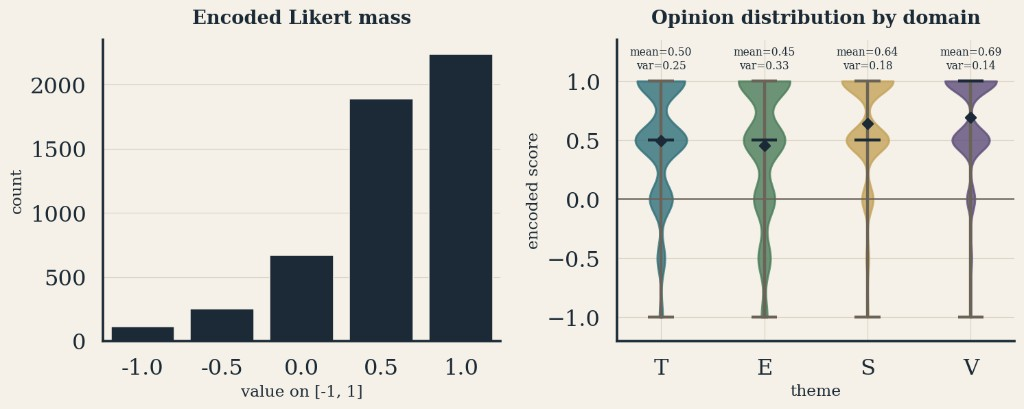
\includegraphics[width=0.72\textwidth]{eda.png}
\caption{Encoded Likert mass (left) and opinion distributions by theme (right).}
\label{fig:eda}
\end{figure}

% ================================================================
\section{Pipeline Followed}

\subsection{Conceptual goal}
Following \citet{maccarron2020}, \citet{dinkelberg2021}, and \citet{maher2020}, we build
two complementary graphs: an \textbf{agent agreement network} (nodes = respondents;
edges = high answer similarity) and an \textbf{attitude co-endorsement network}
(nodes = statements; edges = joint positive endorsement). These are homophily / belief
networks.

\subsection{Agent similarity}
For jointly answered items $F_{ij}$ with $n_{ij}=|F_{ij}|$,
\[
S_{ij}=n_{ij}-\sum_{f\in F_{ij}}|q_{if}-q_{jf}|.
\]
Larger $S_{ij}$ means closer answer profiles. The empirical $S_{ij}$ distribution
(Figure~\ref{fig:simthresh}, left) peaks near~$35$ and is left-skewed; most pairs are only
moderately similar.

\subsection{Threshold selection}
We retain edges with $S_{ij}\ge\theta$ and choose the largest $\theta$ such that the
giant component still covers about \textbf{80\%} of respondents
\citep{dinkelberg2021}. Figure~\ref{fig:simthresh} (right) shows that the giant fraction
stays near~$1$ until roughly~$\theta\approx 20$, then declines; it crosses the $0.8$
target at \textbf{$\theta=41.5$}. That cut sits in the upper tail of $S_{ij}$, so the
kept edges are the strongest agreements only. The resulting agent graph has 87 nodes,
456 edges, density~$0.122$, average degree~$\approx 10.5$, and clustering~$0.45$.

\begin{figure}[htbp]
\centering
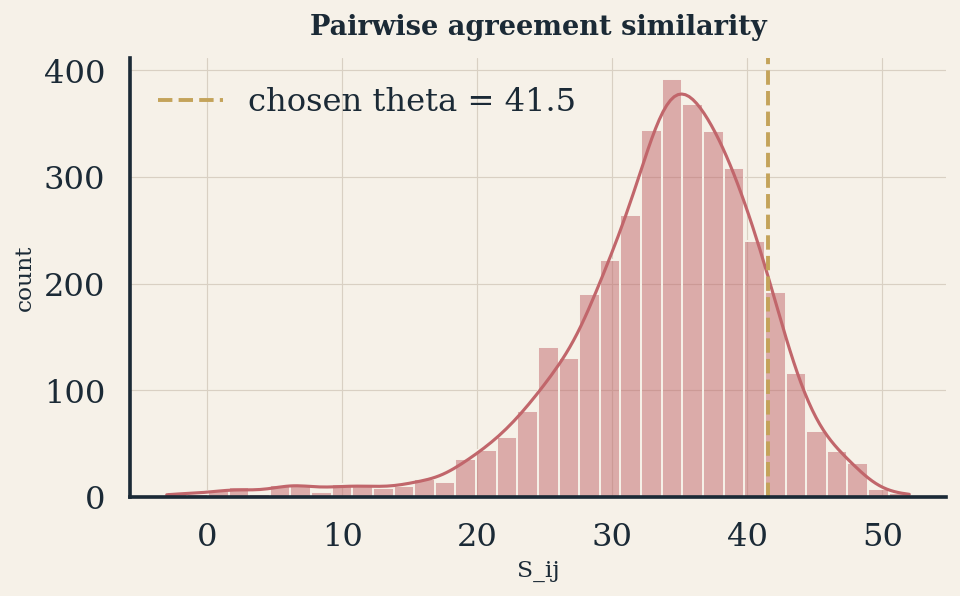
\includegraphics[width=0.4\textwidth]{similarity.png}\hfill
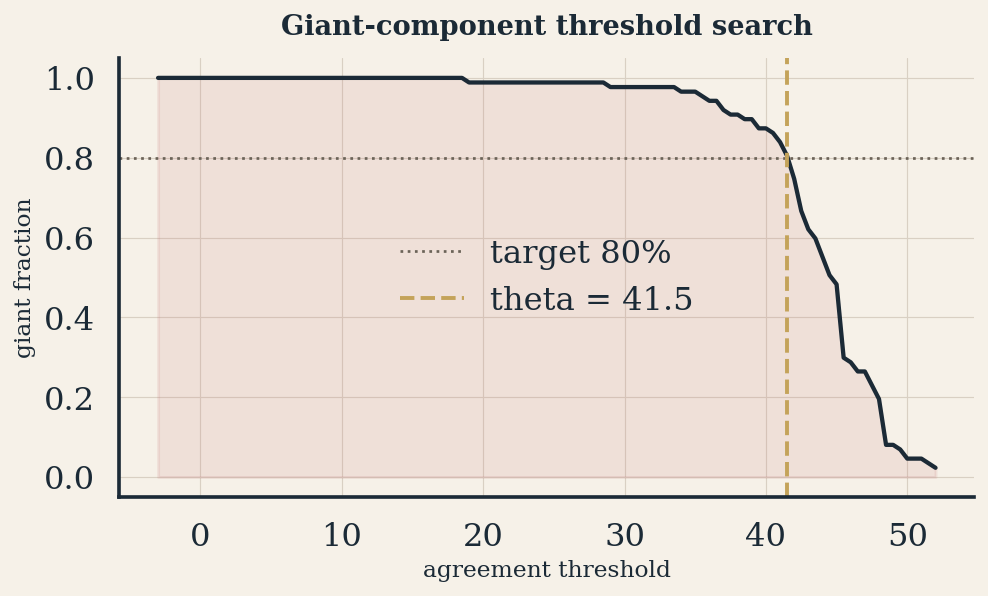
\includegraphics[width=0.4\textwidth]{threshold.png}
\caption{Left: pairwise agreement $S_{ij}$ with chosen $\theta=41.5$.
Right: giant-component fraction vs.\ threshold (target~$80\%$).}
\label{fig:simthresh}
\end{figure}

\subsection{Attitude projection}
Statement pairs use co-endorsement $W_{ab}=\sum_i q_{ia}q_{ib}$ on the $[-1,1]$ encoding.
Strong positive $W_{ab}$ means the two items are routinely affirmed together. We keep
high-$W$ edges for visualization and report the top twenty pairs in
Table~\ref{tab:top20}.

% ================================================================
\section{Analysis and Visualizations}

Network drawings are Cytoscape.js force-directed views (\texttt{cose} layout; edge weight
controls spring strength). Interactive HTML lives under \texttt{figures/cytoscape/}.

\subsection{Agent communities (Louvain)}
Louvain returns 20 communities in total, but only three contain more than one member:
sizes \textbf{37} (C0), \textbf{29} (C1), and \textbf{4} (C2). Modularity is moderate
($Q\approx 0.275$), meaning these communities are only somewhat more internally
connected than a random graph of the same density would be. The other 17 communities are
singletons, and they are exactly the respondents who have zero edges at $\theta=41.5$
(cleared the completeness filter but did not agree strongly enough with anyone else):
nodes with no edges cannot be merged into any group, so Louvain correctly leaves them
alone. In Figure~\ref{fig:louvain}, C0 and C1 sit next to
each other with direct edges running between their members (they are not two separate
components); C2 sits at the boundary between them; the singleton respondents appear as
isolated points scattered around the frame.

\begin{figure}[htbp]
\centering

\includegraphics[width=0.6\textwidth]{agent_louvain.png}
\caption{Agent agreement network colored by Louvain community
(Cytoscape.js, force-directed by edge weight).}
\label{fig:louvain}
\end{figure}

Figure~\ref{fig:comm} plots each community's mean score on each theme. Both C0 and C1
score above zero (the Agree side) on all four themes, so the two communities are not an
agree-versus-disagree split. C0 scores higher than C1 on every theme, most noticeably on
Society (mean~$\approx 0.82$) and Environment (mean~$\approx 0.87$); C1's four theme
means stay in a narrower~$0.42$--$0.56$ range. C2 ($n=4$) has moderate Technology,
Education, and Society means alongside a higher Environment mean. Education has the
lowest mean in all three communities. So C0 and C1 differ in how strongly and
consistently their members agree, not in which direction they lean.

\begin{figure}[htbp]
\centering
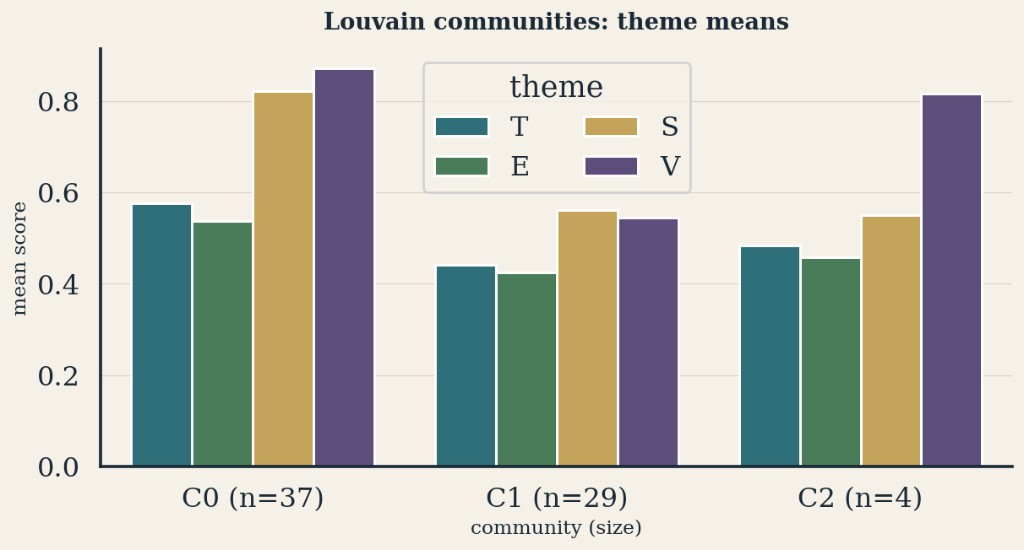
\includegraphics[width=0.58\textwidth]{communities.png}
\caption{Mean theme scores for Louvain communities with size at least~3.}
\label{fig:comm}
\end{figure}

\subsection{Girvan--Newman cut}
Girvan--Newman repeatedly deletes the edge with the highest \emph{betweenness} (the edge
lying on the largest number of shortest paths between other node pairs) until the graph
splits. Applied to the 70-node giant component, the first split is highly uneven:
\textbf{64, 4, and 2} nodes (Figure~\ref{fig:gn}), not two groups of comparable size. The
highest-weight edges (yellow) sit inside the 64-node group, and the two small splinter
groups are attached to it by only one or two low-weight edges, which is exactly why the
algorithm removed those edges first. Together with Louvain's moderate modularity, this
points to one dominant, densely connected group with a few small groups loosely attached,
rather than two comparably sized opposing camps as in the bipolar ANES-style splits
reported in the cited literature.

\begin{figure}[htbp]
\centering

\includegraphics[width=0.6\textwidth]{agent_girvan_newman.png}
\caption{Giant component colored by the Girvan--Newman cut
(Cytoscape.js).}
\label{fig:gn}
\end{figure}

\subsection{Attitude co-endorsement network}
Figure~\ref{fig:att} shows the statement pairs whose co-endorsement $W_{ab}$ clears the
70th-percentile threshold. Society and Environment items form a densely connected core
with many edges among them; several Education and Technology items (e.g.\ E02--E04, E09,
E12, T02, T08, T09) have no surviving edge and appear as isolated nodes. Edges do connect
different themes, but the core is dominated by Society and Environment items together
with two broadly endorsed Education items, continuous learning (E15) and curriculum
update (E11), rather than by an even mix of all four themes.

\begin{figure}[htbp]
\centering

\includegraphics[width=0.6\textwidth]{attitude_themes.png}
\caption{Attitude co-endorsement network colored by theme
(Cytoscape.js).}
\label{fig:att}
\end{figure}

Table~\ref{tab:top20} lists the twenty strongest co-endorsement pairs. \textbf{E15}
appears in 9 of these 20 pairs, more than any other item, pairing with items from all
three other themes; \textbf{E11}, \textbf{V13}, \textbf{V09}, and \textbf{S05} also
recur repeatedly. Six of the twenty pairs connect two items from the same theme (e.g.\
E11--E15, E14--E15, V09--V13, V13--V14); the remaining fourteen connect two different
themes (e.g.\ E15--V13, E15--S05, S05--V13). In other words, respondents who strongly
endorse one broadly worded statement, such as E15 (``continuous learning is
essential''), tend to also strongly endorse the other broadly endorsed statements
regardless of theme label. None of the contested Education items identified in the next
subsection (E02--E04) appears anywhere in this top-20 list.

\begin{table}[H]
\centering
\caption{Top 20 attitude co-endorsement edges ($W_{ab}$).}
\label{tab:top20}
\scriptsize
\setlength{\tabcolsep}{4pt}
\begin{tabular}{@{}rllp{5.6cm}p{5.6cm}r@{}}
\toprule
\# & A & B & Short A & Short B & $W$ \\
\midrule
1  & E11 & E15 & Curricula updated for emerging tech & Continuous learning essential & 63.25 \\
2  & E15 & V13 & Continuous learning essential & Firms accountable for env.\ impact & 62.00 \\
3  & E15 & S05 & Continuous learning essential & Control over personal data & 61.75 \\
4  & E14 & E15 & University--industry collaboration & Continuous learning essential & 61.50 \\
5  & V09 & V13 & Design for reuse/repair & Firms accountable for env.\ impact & 61.25 \\
6  & E15 & V09 & Continuous learning essential & Design for reuse/repair & 61.00 \\
7  & S05 & V13 & Control over personal data & Firms accountable for env.\ impact & 60.50 \\
8  & E10 & E15 & Innovation over rote learning & Continuous learning essential & 60.50 \\
9  & E15 & S11 & Continuous learning essential & Free expression (non-harmful) & 60.00 \\
10 & E15 & V14 & Continuous learning essential & Intl.\ env.\ cooperation & 59.50 \\
11 & E11 & S05 & Curricula updated for emerging tech & Control over personal data & 59.50 \\
12 & E11 & V09 & Curricula updated for emerging tech & Design for reuse/repair & 59.50 \\
13 & V13 & V14 & Firms accountable for env.\ impact & Intl.\ env.\ cooperation & 59.00 \\
14 & E11 & V13 & Curricula updated for emerging tech & Firms accountable for env.\ impact & 59.00 \\
15 & S05 & V09 & Control over personal data & Design for reuse/repair & 58.50 \\
16 & E10 & V13 & Innovation over rote learning & Firms accountable for env.\ impact & 58.25 \\
17 & V09 & V14 & Design for reuse/repair & Intl.\ env.\ cooperation & 58.00 \\
18 & E11 & S11 & Curricula updated for emerging tech & Free expression (non-harmful) & 57.75 \\
19 & E15 & V15 & Continuous learning essential & Protect resources for future gens & 57.50 \\
20 & E10 & V09 & Innovation over rote learning & Design for reuse/repair & 57.25 \\
\bottomrule
\end{tabular}
\end{table}

\subsection{Which statements sit at the core, and which ones bridge}
Degree alone only counts how many edges a node has; two other centrality measures ask
more specific questions about the same attitude network. \textbf{Eigenvector centrality}
scores a statement highly if it connects to other well-connected statements, computed by
repeatedly averaging each node's score with its neighbors' scores until the ranking
stops changing. \textbf{Betweenness centrality} scores a statement highly if it lies on
many shortest paths between other pairs of statements, i.e.\ removing it would make many
other items harder to reach from each other through the network.

The top eigenvector-centrality items are \textbf{E15} (continuous learning, $0.230$),
\textbf{V13} (corporate environmental accountability, $0.225$), \textbf{V09}
(reuse/repair design, $0.219$), \textbf{E11} (curriculum update, $0.219$), and
\textbf{S05} (personal-data control, $0.219$); these are the same five items that
dominate Table~\ref{tab:top20}, confirming that they sit at the well-connected heart of
the network rather than merely appearing in a few strong pairs. The lowest
eigenvector scores belong almost entirely to Technology and Education items (T13, E02,
E03, E04, T03, T02, T08, T01), the same items that are disconnected in
Figure~\ref{fig:att}.

Betweenness centrality tells a different story: \textbf{T14} (social media algorithms
cause polarization) has the highest betweenness ($0.0452$), nearly 50\% higher than the
runner-up V13 ($0.0301$); E15 ($0.0245$), V07 ($0.0245$), and S11 ($0.0212$) follow.
T14's eigenvector score ($0.190$) is noticeably lower than the other top-betweenness
items, so T14 is not itself part of the densely-interconnected core; instead it is the
single most important bridge connecting the more loosely-attached Technology items to
that core. V13, E15, V07, and S11 score highly on both measures, meaning they are
central in two different senses at once: deeply embedded \emph{and} load-bearing bridges.

\subsection{Contested vs.\ community-organizing items}
Variance marks disagreement \emph{content}; shuffle importance
($1-\overline{\mathrm{ARI}}$ after permuting an item vs.\ baseline Louvain) marks
disagreement that \emph{organizes people} (Figure~\ref{fig:items}).

The most contested items are Education-led: \textbf{E04}, \textbf{E03}, \textbf{E02},
then Technology item T08 and Society item S02. No Environment item enters the top
variance list, consistent with V's tight violin in Figure~\ref{fig:eda}. Shuffle
importance also elevates Education (\textbf{E04}, \textbf{E01}) and mixes in T02, S15,
T14, and several V items. So Environment can still structure communities through
\emph{intensity} differences (C0 vs.\ C1) even when raw variance is low, while Education
items are both noisy and structurally decisive.

\begin{figure}[htbp]
\centering
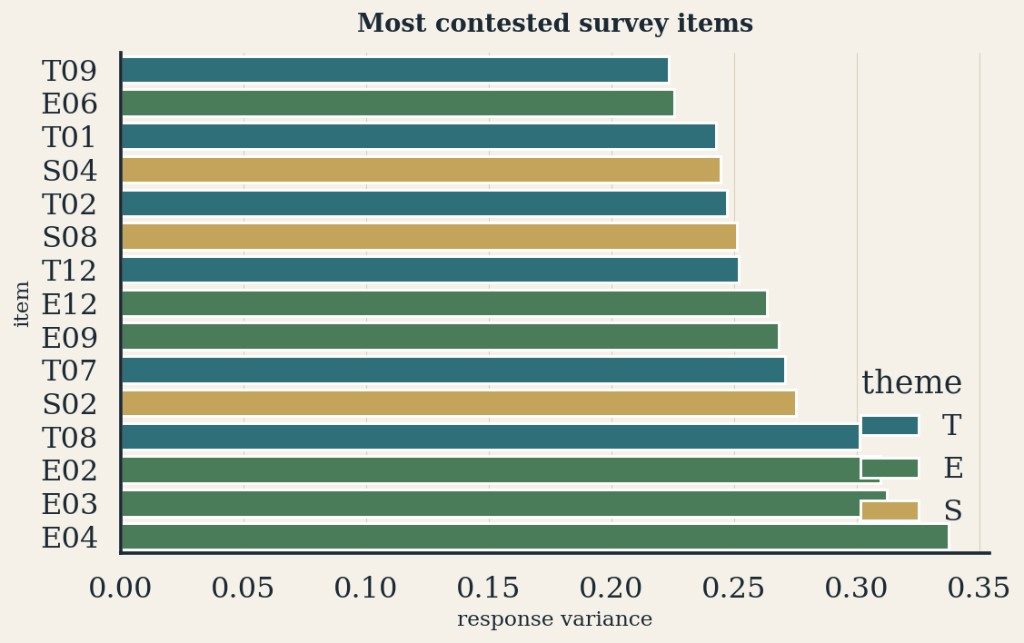
\includegraphics[width=0.4\textwidth]{contested.png}\hfill
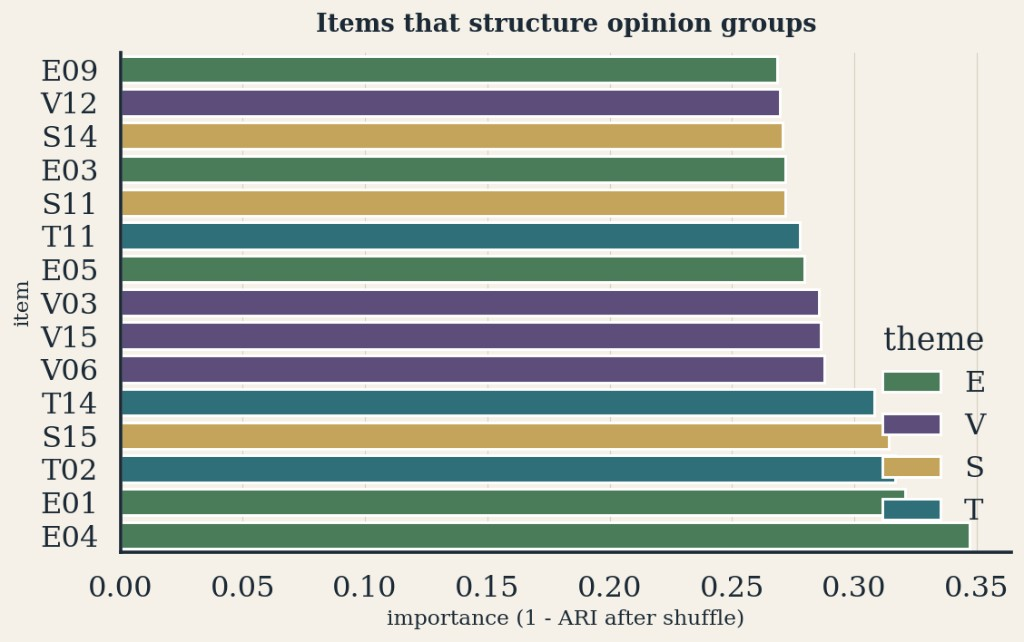
\includegraphics[width=0.4\textwidth]{importance.png}
\caption{Left: highest-variance (most contested) items.
Right: items whose shuffle most disrupts Louvain communities.}
\label{fig:items}
\end{figure}

% ================================================================
\section{Results and Discussion}

Putting the pieces together yields a coherent class portrait.

\begin{enumerate}
  \item \textbf{One connected majority, not separate camps.} Likert mass and theme
  violins show broad Agree-side scores across the class. At $\theta=41.5$, 70 of 87
  respondents ($\sim$80\%) form a single giant component, connected through
  high-agreement edges; the strongest co-endorsement edges among statements
  (Table~\ref{tab:top20}, Figure~\ref{fig:att}) connect mostly Society and Environment
  items.
  \item \textbf{Two neighborhoods that differ in strength, not direction.} Louvain's two
  large communities (C0, 37 members; C1, 29 members) are both positive on every theme,
  but C0's means run higher, especially on Society and Environment. Girvan--Newman's
  uneven 64/4/2 split, together with Louvain's moderate modularity ($Q=0.275$), rules out
  a two-camp, opposed-ideology structure.
  \item \textbf{Education items account for most of the disagreement.} Education has the
  lowest mean and highest variance among the four themes; its items dominate the
  contested-item ranking and the structural-importance ranking (E04, E03, E02; E04, E01)
  in Figure~\ref{fig:items}. These same contested items do not appear among the strongest
  co-endorsement pairs in Table~\ref{tab:top20}, which instead feature the two
  near-consensus Education items E15 and E11.
  \item \textbf{A small set of statements is endorsed together far more than the rest.}
  The attitude network (Figure~\ref{fig:att}) and Table~\ref{tab:top20} show that
  sustainability items (V09, V13, V14, V15), the data-control item (S05), and the two
  consensus Education items (E15, E11) are co-endorsed much more strongly than other item
  combinations. Technology items and the contested Education items sit on the periphery
  of the network or are disconnected entirely after thresholding.
\end{enumerate}

\subsection{What the network view adds}
Computing theme means alone would show only that every theme's average score is
positive. It would not show that 80\% of respondents form one connected group at a
principled agreement threshold; that this group splits further into two neighborhoods
differing in agreement strength rather than direction; that some items are contested
(high variance) while a partly different set of items is structurally decisive (high
shuffle-importance); or that specific statements are co-endorsed together far more than
others. The MacCarron/Dinkelberg pipeline recovers all of this by turning the Likert
table into a graph that can be thresholded, partitioned, and stress-tested: students
share a Society/Environment agreement core, while education practice (and related
Technology items) account for most of the remaining disagreement.

A practical reading for the class is therefore not ``students disagree about the
environment,'' but ``students largely co-endorse sustainability and data-rights
statements, and diverge more when asked how universities and AI should teach.'' That
distinction is visible only once agreement edges, community profiles, contestation, and
co-endorsement hubs are read together.

% ================================================================
\section{Individual Contribution}

\begin{table}[H]
\centering
\small
\begin{tabular}{@{}p{3.6cm}p{11.0cm}@{}}
\toprule
\textbf{Member} & \textbf{Contribution} \\
\midrule
Kushal Balabhadruni &
Section~3: designed the $[-1,0.5,0,0.5,1]$ Likert encoding and the missing-vs.-neutral
rule for blanks/\texttt{No Comments}; applied the 50\% completeness filter (96
$\rightarrow$ 87 respondents); computed the per-theme means/variances and built
Figure~\ref{fig:eda} (encoded Likert mass and theme violins). \\
\midrule
Rohit Jeswanth &
Section~4 and Section~5.1, 5.2, 5.5: derived the agreement score $S_{ij}$ and ran the
threshold scan that fixed $\theta=41.5$ against the 80\% giant-component target
(Figure~\ref{fig:simthresh}); computed Louvain modularity ($Q=0.275$) and the
Girvan--Newman betweenness cut (64/4/2 split); exported the agent-network GraphML used
for Figures~\ref{fig:louvain}--\ref{fig:gn}; ran the response-variance and
shuffle-based item-importance rankings behind Figure~\ref{fig:items}. \\
\midrule
Vishak Kashyap K &
Section~4.4 and Section~5.3--5.4: defined the co-endorsement weight $W_{ab}$ and built
the attitude network and Table~\ref{tab:top20} top-20 ranking; computed eigenvector and
betweenness centrality on the attitude network; produced the Cytoscape.js force-directed
renderings (Figures~\ref{fig:louvain}, \ref{fig:gn}, \ref{fig:att}); assembled the LaTeX
report and repository layout/README. \\
\bottomrule
\end{tabular}
\end{table}

% ================================================================
\section{References}
\renewcommand{\refname}{}
\vspace{-1.8em}
\begin{thebibliography}{9}
\bibitem[MacCarron et~al.(2020)]{maccarron2020}
MacCarron, P., Maher, P. J., and Quayle, M. (2020). Identifying opinion-based groups from
survey data: a bipartite network approach. arXiv:2012.11392.
\bibitem[Dinkelberg et~al.(2021)]{dinkelberg2021}
Dinkelberg, A., MacCarron, P., Maher, P. J., and Quayle, M. (2021). Detect opinion-based
groups and reveal polarisation in survey data. arXiv:2104.14427.
\bibitem[Maher et~al.(2020)]{maher2020}
Maher, P. J., MacCarron, P., and Quayle, M. (2020). Mapping public health responses with
attitude networks. \emph{British Journal of Social Psychology}.
\end{thebibliography}

\end{document}
